\section{Derivation of the Time Dilation Formula within VAM}
\label{sec:appendix:1}

\begin{abstract}
    We present a unified time dilation formula derived from the Vortex \AE{}ther Model (VAM), a fluid-dynamic reformulation of gravitation and mass-energy interactions. Unlike General Relativity, where mass and curvature govern clock rates, VAM attributes gravitational phenomena to quantized vorticity, \ae{}ther circulation, and swirl-induced pressure gradients. The proposed equation replaces the Schwarzschild and Kerr metric terms with vortex core tangential velocities, swirl angular frequencies, and an effective mass derived from exponentially decaying \ae{}ther density. A hybridization mechanism smoothly interpolates between vortex-scale gravity and classical Newtonian coupling at macroscopic distances. The final expression captures six physical effects within one coherent framework: (1) vortex-induced mass generation via circulation and helicity, (2) bubble-like volume expansion due to internal irrotational flow, (3) acceleration of this flow under compression, (4) thermal-like energy response from swirl speedup, (5) relativistic time dilation from \ae{}ther puncture during motion, and (6) swirl-based core-local time. The result is a mathematically robust, numerically testable model that unifies quantum vortex dynamics with gravitational time effects and remains non-singular across all radial domains.
\end{abstract}

\section*{Introduction}
In General Relativity (GR), time dilation arises from mass and angular momentum, expressed through the Schwarzschild and Kerr metrics. In contrast, the Vortex \ae{}ther Model (VAM) reformulates this effect in terms of vorticity, internal circulation, and local \ae{}ther properties. Gravitational effects are no longer sourced by geometric curvature but by fluid-dynamic structures in an inviscid, rotational medium.

This appendix derives a unified time dilation expression from first principles of vortex mechanics, incorporating:

\begin{itemize}
    \item Vortex-induced mass generation through circulation,
    \item Frame-dragging from swirl angular momentum,
    \item Bubble-like volume expansion resembling thermodynamic gas laws,
    \item Exponential decay of vorticity and pressure with distance,
    \item Smooth hybridization with classical Newtonian gravity at large $r$.
\end{itemize}

\subsection{Unified Time Dilation in VAM}
We define the time dilation factor between the local Chronos-Time $\tau$ and the absolute Aith\=er-Time $\mathcal{N}$ as:

\begin{equation}
    \boxed{
        \frac{d\tau}{d\mathcal{N}} = \sqrt{
            1
            - \frac{2 G_{\text{hybrid}}(r) M_{\text{hybrid}}(r)}{r c^2}
            - \frac{C_e^2}{c^2} e^{-r/r_c}
            - \frac{C_e^2}{r_c^2 c^2} e^{-r/r_c}
        }}
    \label{eq:final_vam_td}
\end{equation}

Here, $\tau$ is the local proper time tracked within the vortex region (Chronos-Time), and $\mathcal{N}$ is the background causal time (Aith\=er-Time). The terms reflect rotational energy, vorticity-induced gravity, and pressure gradients.

\subsection{Decomposition in Standard Coordinate Time}
We can recast equation~\eqref{eq:final_vam_td} in terms of standard coordinate time $t$ to interpret local clock behavior:

\begin{equation}
    \frac{d\tau}{dt} = \sqrt{
        1
        - \frac{C_e^2}{c^2} e^{-r/r_c}
        - \frac{2 G_\text{swirl} M_\text{eff}(r)}{r c^2}
        - \beta \Omega^2
    }
\end{equation}

Each term corresponds to a distinct physical source:

\begin{itemize}
    \item \textbf{(1) Local Swirl --- Core Rotation Delay}
    \[
        \frac{C_e^2}{c^2} e^{-r/r_c}
    \]
    Caused by the vortex core's tangential velocity $C_e$ and the exponential decay scale $r_c$. Represents time delay from local \ae{}ther rotation.

    \item \textbf{(2) Vorticity-Induced Gravitation --- Swirl Mass Equivalent}
    \[
        \frac{2 G_\text{swirl} M_\text{eff}(r)}{r c^2}
    \]
    Analogous to gravitational redshift but sourced by vorticity-derived effective mass and the swirl-specific coupling constant $G_\text{swirl}$.

    \item \textbf{(3) Frame Dragging --- Macroscopic Inertial Delay}
    \[
        \beta \Omega^2
    \]
    Arises from large-scale rotational motion. With $\Omega = \Gamma / (2\pi r^2)$ and $\beta = 1/c^2$, this models inertial time delay from \ae{}theric circulation.
\end{itemize}

\paragraph{Note on $G_\text{swirl}$:}
The gravitational coupling in Eq.~\eqref{eq:final_vam_td} uses a vorticity-derived form (see Appendix~\ref{appendix:SwirlGravity}),
\[
    G_\text{swirl} = \frac{C_e c^5 t_p^2}{2 F_{\text{max}} r_c^2}
\]
providing a fluid-dynamical analog to Newton's constant based on swirl energy density and æther properties.


\subsection{Expanded Derivation: Rotational Energy as Time Delay Source}

\subsubsection{Energetic Derivation}

A clock embedded in a vortex experiences delay due to the kinetic energy of rotation:

\begin{equation}
    \frac{d\tau}{dt} = \left(1 + \frac{1}{2} \beta I \Omega^2 \right)^{-1},
\end{equation}

where $I$ is moment of inertia, $\Omega$ is angular velocity, and $\beta = 1/c^2$. For a ring mass $I = m r^2$:

\[
    \frac{1}{2} \beta I \Omega^2 = \frac{1}{2} \frac{r^2 \Omega^2}{c^2}
\]

\subsubsection{Hydrodynamic Derivation: Bernoulli Pressure Deficit}

From Bernoulli's law:
\[
    \frac{1}{2} \rho v^2 + p = \text{const.}, \quad \Rightarrow \Delta p = -\frac{1}{2} \rho \Omega^2 r^2
\]
Clock rate varies with enthalpy:
\[
    \frac{d\tau}{dt} \approx \frac{H_\text{ref}}{H_\text{loc}} \approx \left(1 + \frac{1}{2} \beta I \Omega^2 \right)^{-1}
\]

\subsubsection{Interpretation Across Domains}
\begin{itemize}
    \item \textbf{Mechanical:} Delay tracks angular kinetic energy.
    \item \textbf{Hydrodynamic:} Time slows in pressure-depleted zones.
    \item \textbf{Thermodynamic:} Entropy increase maps to time dilation.
\end{itemize}

\subsection{Hybridization of Gravitational Coupling}
To reconcile short- and long-range predictions:
\[
    \mu(r) = \exp\left(-\frac{r^2}{R_0^2}\right), \quad R_0 \sim 10^{-12} \, \mathrm{m}
\]
\begin{align*}
    G_{\text{hybrid}}(r) &= \mu(r) \, G_{\text{swirl}} + (1 - \mu(r)) \, G \\
    M_{\text{hybrid}}(r) &= \mu(r) \, M_\text{eff}^\text{VAM}(r) + (1 - \mu(r)) \, M
\end{align*}

\subsection{Effective VAM Mass}
Assuming exponentially decaying \ae{}ther density:
\[
    \rho_\text{\ae}(r) = \rho_0 e^{-r / r_c}
\]
The effective mass becomes:
\[
    M_\text{eff}^\text{VAM}(r) = 4\pi \rho_0 r_c^3 \left(2 - \left(2 + \frac{r}{r_c} \right) e^{-r/r_c} \right)
\]

\begin{figure}[H]
    \centering
    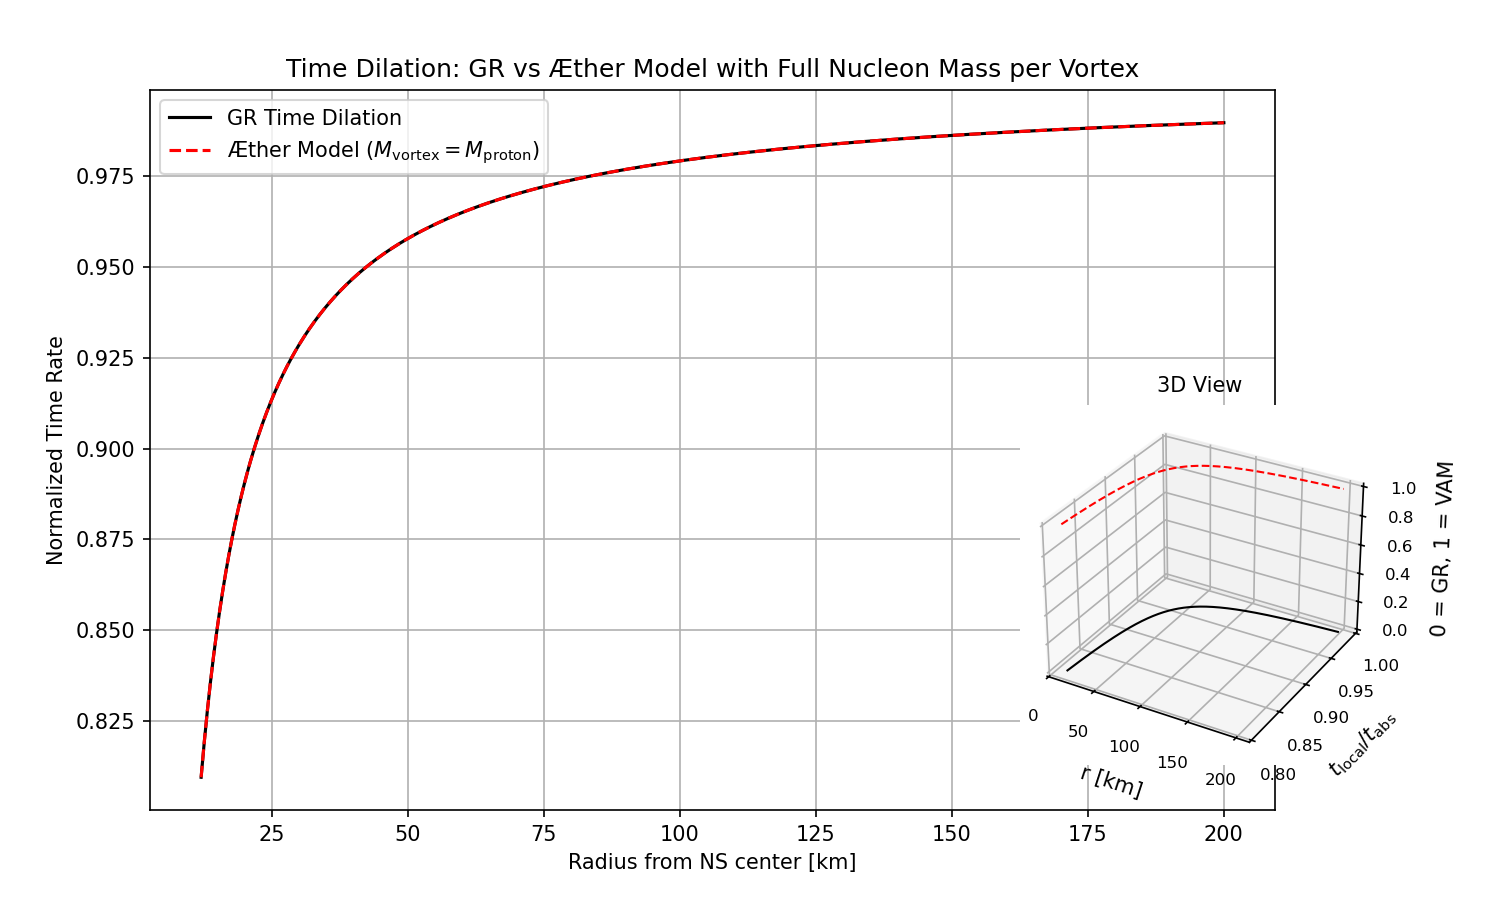
\includegraphics[width=0.85\textwidth]{images/07-TimeDilationGRVsVAM}
    \caption{\textbf{Comparison of Time Dilation Models:} GR's metric-based formula $\sqrt{1 - 2GM/(rc^2)}$ is contrasted with VAM's fluid-based dilation. The divergence at short radii highlights vortex dominance.}
    \label{fig:GRvsVAMTimeDilation}
\end{figure}


The above equation is analogous to relativistic formulas, but has a fluid mechanics origin. Experimentally, components of this formula can be found in time dilation of GPS clocks (gravity), Lense-Thirring effects (rotation), and hypothetical laboratory measurements of nuclear rotations on the quantum or vortex scale.

\section*{Conclusion}
This equation synthesizes all prior VAM elements: vortex helicity, bubble boundaries, circulation-induced gravity, and exponential suppression of short-range fields. It remains finite, matches classical predictions at macroscopic scales, and enables numerical probing at quantum scales.

\subsection{Constants and Variables}

\begin{table}[H]
      \centering
      \footnotesize
      \begin{tabular}{llll}
          \toprule
          \textbf{Symbol} & \textbf{Meaning} & \textbf{Value / Expression} & \textbf{Units} \\
          \midrule
        $G_{\text{hybrid}}(r)$ & Hybrid gravitational constant (VAM/GR) & $\mu(r) G_{\text{swirl}} + (1 - \mu(r)) G$ & $\text{m}^3\,\text{kg}^{-1}\,\text{s}^{-2}$ \\
        $\mu(r)$ & Vortex-to-classical transition function & $e^{-r^2 / R_0^2}$, $R_0 = 1.0 \times 10^{-12}\,\text{m}$ & unitless \\
        $G$ & Newtonian gravitational constant & $6.67430 \times 10^{-11}$ & $\text{m}^3\,\text{kg}^{-1}\,\text{s}^{-2}$ \\
        $G_{\text{swirl}}$ & Swirl-induced gravitational constant & $\dfrac{C_e c^5 t_p^2}{2 F_{\max} r_c^2}$ & $\text{m}^3\,\text{kg}^{-1}\,\text{s}^{-2}$ \\
        $M_{\text{hybrid}}(r)$ & Hybrid effective mass & $\mu(r) M_\text{eff}^\text{VAM}(r) + (1 - \mu(r)) M$ & $\text{kg}$ \\
        $M_\text{eff}^\text{VAM}(r)$ & Vortex effective mass & $4\pi \rho_\text{\ae} r_c^3 \left[ 2 - (2 + \frac{r}{r_c}) e^{-r/r_c} \right]$ & $\text{kg}$ \\
        $\rho_\text{\ae}$ & Æther density & $3.89343583 \times 10^{18}$ & $\text{kg}\cdot\text{m}^{-3}$ \\
        $r_c$ & Core radius (Coulomb scale) & $1.40897017 \times 10^{-15}$ & $\text{m}$ \\
        $C_e$ & Core tangential velocity & $1.09384563 \times 10^{6}$ & $\text{m}\cdot\text{s}^{-1}$ \\
        $t_p$ & Planck time & $5.391247 \times 10^{-44}$ & $\text{s}$ \\
        $F_{\max}$ & Maximum force & $29.053507$ & $\text{N}$ \\
        $\left(\frac{C_e}{r_c}\right)^2$ & Squared swirl angular frequency ($\Omega^2$) & $6.02367430 \times 10^{42}$ & $\text{s}^{-2}$ \\
        $c$ & Speed of light & $2.99792458 \times 10^8$ & $\text{m}\cdot\text{s}^{-1}$ \\
          \bottomrule
      \end{tabular}
    \caption{Key symbols and constants in the VAM time dilation equation.}
      \label{tab:time_dilation_symbols}
  \end{table}

\begin{table}[H]
    \centering
    \footnotesize
    \begin{tabular}{llll}
        \toprule
        \textbf{Symbol} & \textbf{Meaning} & \textbf{Description} & \textbf{Value (if constant)} \\
        \midrule
        $\Delta t$ & Reference time & Clock far from gravitating body & -- \\
        $t_\text{adjusted}$ & Local time & Time experienced near the vortex structure & -- \\
        $r$ & Radial coordinate & Distance from the vortex core & m \\
        $r_c$ & Vortex core radius & Characteristic decay scale & $1.40897017 \times 10^{-15}$ m \\
        $C_e$ & Vortex tangential velocity & Maximal edge swirl velocity & $1.09384563 \times 10^6$ m/s \\
        $\rho_\text{\ae}$ & Æther density & Fluid density of the æther & $\sim 3.89 \times 10^{18}$ J/m$^3$ \\
        $c$ & Speed of light & Vacuum light speed & $2.99792458 \times 10^8$ m/s \\
        $G$ & Newton's constant & Classical gravity & $6.67430 \times 10^{-11}$ m$^3$/kg/s$^2$ \\
        $F_{\text{max}}$ & Max force & From Planck-scale dynamics & $29.053507$ N \\
        $t_p$ & Planck time & Quantum gravity scale & $5.391247 \times 10^{-44}$ s \\
        $G_\text{swirl}$ & Vortex gravity coupling & $C_e c^5 t_p^2 / (2 F_{\text{max}} r_c^2)$ & -- \\
        $M$ & Macroscopic mass & Classical object mass (e.g., proton mass) & $1.67262192 \times 10^{-27}$ kg \\
        $M_{\text{eff}}^\text{VAM}(r)$ & VAM mass & Mass from vorticity energy & derived \\
        $M_{\text{hybrid}}(r)$ & Hybrid mass & Smooth transition between VAM and GR & -- \\
        $G_{\text{hybrid}}(r)$ & Hybrid gravity constant & Smooth transition between $G$ and $G_\text{swirl}$ & -- \\
        $\mu(r)$ & Hybrid blending function & $\mu(r) = \exp\left(-\frac{r^2}{R_0^2}\right),\ R_0 \sim 10^{-12}$ m & dimensionless \\
        $e^{-r/r_c}$ & Vorticity decay & Exponential suppression term & -- \\
        \bottomrule
    \end{tabular}
    \caption{Explanation of variables in Equation~\ref{eq:final_vam_td}.}
    \label{tab:time_dilation_variables}
\end{table}